\documentclass[preview]{standalone}

\usepackage{amsmath}
\usepackage{amssymb}
\usepackage{stellar}
\usepackage{definitions}
\usepackage{blkarray}
\usepackage{tikz}

\begin{document}

\id{graphs}
\genpage

\section{Definitions}

\begin{snippetdefinition}{graph-definition}{Graph}
    A \textit{graph} is a tuple \((V,E)\) where
    \begin{itemize}
        \item \(V\) is a set of \textit{vertices} or \textit{nodes};
        \item \(E \subseteq \{\{x,y\} \,|\, x,y \in V \land x \neq y\}\) is a set of \textit{edges}.
    \end{itemize}
\end{snippetdefinition}

\begin{snippetdefinition}{graph-adjacent-vertices-definition}{Adjacent vertices}
    Let \(G=(V,E)\) be a \snippetref[graph-definition][graph].
    Two vertices \(v_1,v_2 \in V\) are \textit{adjacent}
    if \(\{v_1,v_2\} \in E\).
\end{snippetdefinition}

\begin{snippetdefinition}{graph-adjacent-edges-definition}{Adjacent edges}
    Let \(G=(V,E)\) be a \snippetref[graph-definition][graph].
    Two distinct edges \(e_1, e_2 \in E\) are \textit{adjacent}
    if \(e_1 \intersection e_2 \neq \emptyset \).
\end{snippetdefinition}

\begin{snippetdefinition}{graph-order-definition}{Order of a graph}
    Let \(G=(V,E)\) be a \snippetref[graph-definition][graph].
    The \textit{order} of \(G\) is the number of vertices \(\cardinality{V}\).
\end{snippetdefinition}

\begin{snippetdefinition}{graph-size-definition}{Size of a graph}
    Let \(G=(V,E)\) be a \snippetref[graph-definition][graph].
    The \textit{size} of \(G\) is the number of edges \(\cardinality{E}\).
\end{snippetdefinition}

\section{Adjacency Matrices}

\begin{snippetdefinition}{adjacency-matrix-definition}{Adjacency Matrix}
    A finite \snippetref[graph-definition][graph] can be represented by a square matrix
    \(n \times n\) where \(n\) is the number of vertices.

    \begin{center}
        \begin{minipage}[r]{6cm}
            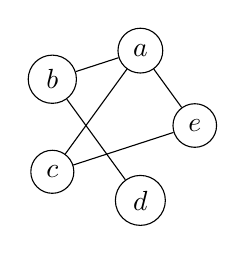
\begin{tikzpicture}[main/.style = {draw, circle}]
                \foreach \x [count = \xi] in {a,b,c,d,e} {
                    \node[main] (\xi) at
                        ({1 * cos(360 / 5 * \xi)}, {1 * sin(360 / 5 * \xi)})
                        {\(\x\)};
                }
            
                \draw (1) -- (2);
                \draw (1) -- (3);
                \draw (1) -- (5);
                \draw (2) -- (4);
                \draw (5) -- (3);
            \end{tikzpicture} 
        \end{minipage}
        \begin{minipage}[l]{6cm}
            A=
            \begin{blockarray}{cccccc}
                & a & b & c & d & e \\
                \begin{block}{c(ccccc)}
                a & 0 & 1 & 1 & 0 & 1 \\
                b & 1 & 0 & 0 & 1 & 0 \\
                c & 1 & 0 & 0 & 0 & 1 \\
                d & 0 & 1 & 0 & 0 & 0 \\
                e & 1 & 0 & 1 & 0 & 0 \\
                \end{block}
            \end{blockarray}
        \end{minipage}
    \end{center}

    Every row and column represents a vertex. \(1\) means
    that the two vertices are adjacent, \(0\) otherwise. The diagonal of this matrix
    will always e \(0s\) since no vertice is adjacent to itself
    and \(A=A^\transpose\)
\end{snippetdefinition}

\section{Degree}

\begin{snippetdefinition}{graph-vertex-degree}{Degree}
    Let \(G=(V,E)\) be a \snippetref[graph-definition][graph]. The \textit{degree} of a vertex \(v \in V\), denoted \(deg(v)\) is defined
    as the numbers of edges in \(E\) that are incident on \(v\).
\end{snippetdefinition}

\begin{snippetproposition}{graph-sum-of-degrees}{Sum of degrees of graph}
    Let \(G=(V,E)\) be a \snippetref[graph-definition][graph].
    The sum of the \snippetref[graph-vertex-degree][degrees] of all vertices is equals to twice the number of edges.
    \[
        \sum_{v\in V}deg(v)=2|E|
    \]
\end{snippetproposition}

\section{Types of graphs}

\begin{snippetdefinition}{null-graph-definition}{Null graph}
    The \textit{null graph} is the \snippetref[graph-definition][graph] \((\emptyset, \emptyset)\).
\end{snippetdefinition}

\begin{snippetdefinition}{empty-graph-definition}{Empty graph}
    Let \(G=(V, E)\) be a \snippetref[graph-definition][graph].
    \(G\) is an \textit{empty graph} if \(V = \emptyset\).
\end{snippetdefinition}

\begin{snippetdefinition}{trivial-graph-definition}{Trivial graph}
    Let \(G=(V, E)\) be a \snippetref[graph-definition][graph].
    \(G\) is a \textit{trivial graph} if \(|V| = 1\).
\end{snippetdefinition}

\section{Subgraphs}

\begin{snippetdefinition}{improper-subgraph-definition}{Improper subgraph}
    Let \(G=(V_G, E_G)\) and \(H=(V_H,E_H)\) be \snippetref[graph-definition][graphs]. \\
    \(H\) is an \textit{improper subgraph} of \(G\), denoted \(H \subseteq G\),
    if \(V_H \subseteq V_G \land E_H \subseteq E_G\).
\end{snippetdefinition}

\begin{snippetdefinition}{proper-subgraph-definition}{Proper subgraph}
    Let \(G=(V_G, E_G)\) and \(H=(V_H,E_H)\) be \snippetref[graph-definition][graphs]. \\
    \(H\) is a \textit{proper subgraph} of \(G\), denoted \(H \subset G\),
    if \(V_H \subset V_G \land E_H \subset E_G\).
\end{snippetdefinition}

\begin{snippetdefinition}{spanning-subgraph-definition}{Spanning subgraph}
    Let \(G=(V_G, E_G)\) and \(H=(V_H,E_H)\) be \snippetref[graph-definition][graphs]. \\
    \(H\) is a \textit{spanning subgraph} of \(G\)
    if \(V_H = V_G \land E_H \subseteq E_G\).
\end{snippetdefinition}

\begin{snippetdefinition}{vertex-induced-subgraph-definition}{Vertex-Induced subgraph}
    Let \(G=(V, E)\) be a \snippetref[graph-definition][graph] and \(S \subseteq V\).
    The \textit{vertex-induced subgraph} of \(G\) by \(S\)
    is the subgraph of \(G\), denoted \(G[S]\), with vertices \(S\) and edges
    such that any two vertices \(v_1, v_2 \in G[S]\)
    are adjacent iff they are adjacent in \(G\).
    That is, \(G[S]\) has some vertices of \(G\) that are adjacent iff they are adjacent in \(G\).
\end{snippetdefinition}

\begin{snippetdefinition}{edge-induced-subgraph-definition}{Edge-Induced subgraph}
    Let \(G=(V, E)\) be a \snippetref[graph-definition][graph] and \(S \subseteq E\).
    The \textit{edge-induced subgraph} of \(G\) by \(S\)
    is the subgraph of \(G\), denoted \(G[S]\), with edges \(S\) and vertices
    such that for any vertex \(v \in G[S]\), \(v \subset e\)
    for some edge \(e \in S\).
    That is, \(G[S]\) has some edges of \(G\) and only vertices that are incident on said vertices.
\end{snippetdefinition}

\section{Paths}

\begin{snippetdefinition}{walk-definition}{Walk}
    Let \(G=(V, E)\) be a \snippetref[graph-definition][graph].
    A \textit{walk} on \(G\) is a sequence of vertices in \(V\),
    where each consecutive pair of vertices are adjacent.
\end{snippetdefinition}

\begin{snippetdefinition}{trial-definition}{Trail}
    Let \(G=(V, E)\) be a \snippetref[graph-definition][graph].
    A \textit{trail} on \(G\) is a sequence of vertices in \(V\),
    where each consecutive pair of vertices are adjacent but no edge can be traversed multiple times.
\end{snippetdefinition}

\begin{snippetdefinition}{path-definition}{Path}
    Let \(G=(V, E)\) be a \snippetref[graph-definition][graph].
    A \textit{path} on \(G\) is a sequence of vertices in \(V\),
    where each consecutive pair of vertices are adjacent but no vertex can be traversed multiple times.
\end{snippetdefinition}

\begin{snippetdefinition}{ciclic-path-definition}{Cycle}
    Let \(P\) be a \snippetref[path-definition][path] on \(G=(V, E)\).
    The path is said to be \textit{cycle} if it starts and end at the same vertex.
\end{snippetdefinition}

\begin{snippetdefinition}{simple-path-definition}{Simple path}
    Let \(P\) be a \snippetref[path-definition][path] on \(G=(V, E)\).
    The path is said to be \textit{simple} if every vertex in it is distinct.
\end{snippetdefinition}

\begin{snippetdefinition}{connected-path-definition}{Connected path}
    Let \(G=(V, E)\) be a \snippetref[graph-definition][graph].
    The graph is said to be \textit{connected} if there exist
    at least a \snippetref[path-definition][path] between any pair of vertices.
\end{snippetdefinition}

% [ https://youtu.be/728bZWwTbf8?list=PLztBpqftvzxXBhbYxoaZJmnZF6AUQr1mH ; ... ]
% https://courses.maths.ox.ac.uk/pluginfile.php/93815/mod_resource/content/3/GraphTheoryPartA-notes-2023.pdf

\end{document}